\chapter{Kerr black hole}
\label{s:ker}
\index{Kerr!black hole}

\minitoc

\section{Introduction}

\section{The Kerr solution}

\subsection{Expression in Boyer-Lindquist coordinates} \label{s:ker:expr_BL}

The Kerr solution depends on two constant real non-negative parameters:
\begin{itemize}
\item the \defin{mass parameter}\index{mass!parameter of Kerr solution} $m > 0$, to be
interpreted in Sec.~?? as the spacetime total mass;
\item the \defin{spin parameter}\index{spin!parameter of Kerr solution} $a \geq 0 $,
to be interpreted in Sec.~?? as the reduced angular momentum  $a=J/m$, $J$ being the
spacetime total angular momentum.
\end{itemize}
In this part, we focus on Kerr solutions for which
\be \label{e:ker:a_lower_m}
    0 < a < m .
\ee
The Kerr solution is usually presented in the so-called
\defin{Boyer-Lindquist coordinates}\index{Boyer-Lindquist coordinates}
$(t,r,\th,\ph)$. Except for the standard singularities of the
spherical coordinates $(\th,\ph)$ on $\SS^2$ at $\theta\in\{0,\pi\}$,
we may consider that the Boyer-Lindquist coordinates cover the manifold
$\R^2\times\SS^2$, with $t$ spanning $\R$, $r$
spanning\footnote{NB: $r$ does not only span $(0,+\infty)$ as in the case of
the standard spherical coordinates $(r,\th,\ph)$ on $\R^3$.} $\R$ and
$\th$ spanning $(0,\pi)$ and $\ph$ spanning $(0,2\pi)$. Hence
$(t,r)$ is a Cartesian chart covering $\R^2$ and $(\th,\ph)$ is the standard
spherical chart of $\SS^2$.

\begin{figure}
\centerline{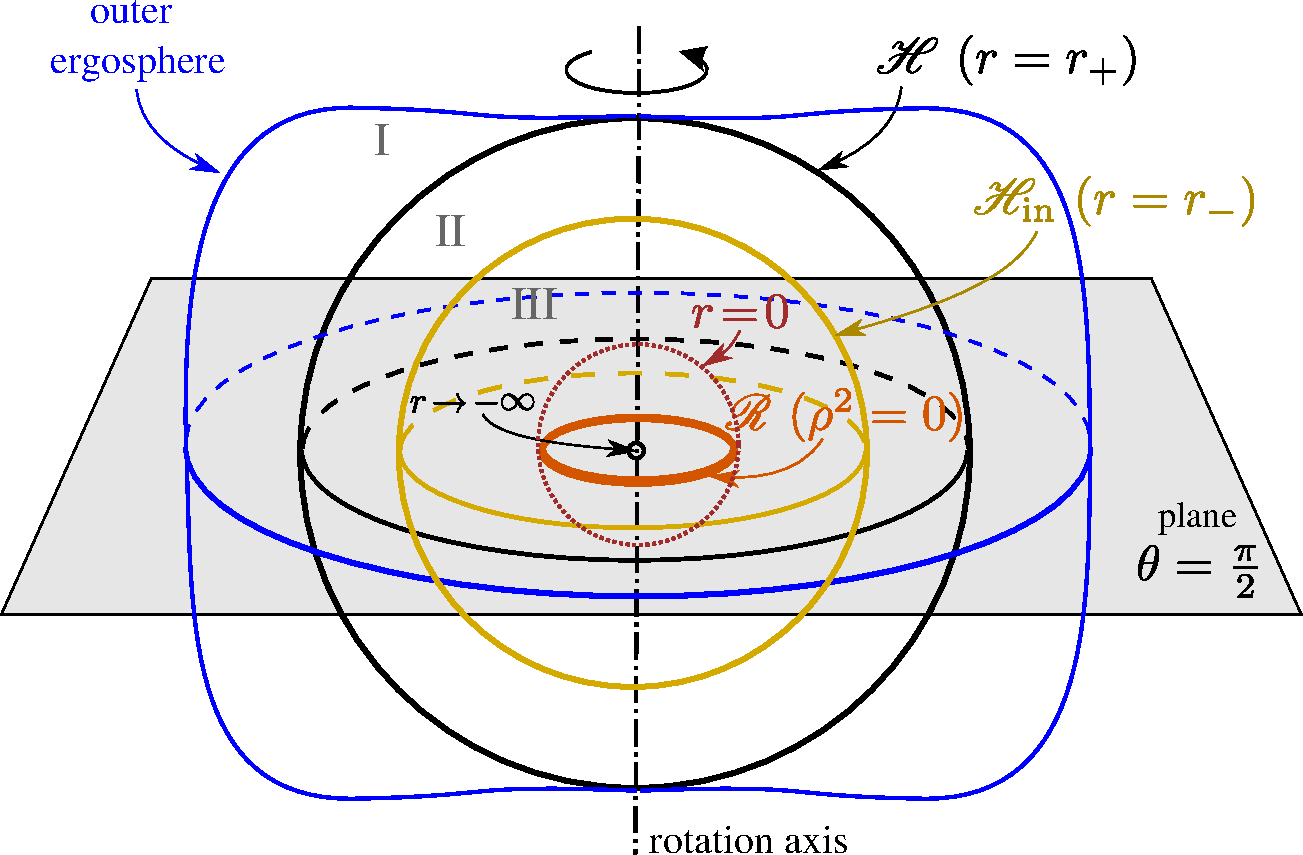
\includegraphics[width=0.8\textwidth]{ker_spher_view.pdf}}
\caption[]{\label{f:ker:spher_view} \footnotesize
A view of a section $t=\mathrm{const}$ of $\mathbb{R}^2\times\mathbb{S}^2$
in terms of the coordinates $(R,\th,\ph)$, with $R:=\mathrm{e}^r$,
so that the region $r\rightarrow -\infty$
is reduced to a single point at the centre of all the pictured spheres.}
\end{figure}


In this section, let us choose the spacetime manifold the open subset $\M_{\rm BL}$
of $\mathbb{R}^2\times\mathbb{S}^2$ formed by the disjoint union of
the following three components (cf. Fig.~\ref{f:ker:spher_view}):
\begin{subequations}
\begin{align}
    \M_{\rm BL} & :=  \M_{\rm I} \cup \M_{\rm II} \cup \M_{\rm III} , \\
    \M_{\rm I} & :=  \R\times(r_+,+\infty)\times\SS^2 \label{e:ker:def_M_I}\\
    \M_{\rm II} & :=  \R\times(r_-,r_+)\times\SS^2 \\
    \M_{\rm III} & :=  \R\times(-\infty,r_-)\times\SS^2 \setminus \ring, \label{e:ker:def_M_III}
\end{align}
\end{subequations}
where
\be \label{e:ker:def_r_pm}
    \encadre{r_+ := m + \sqrt{m^2-a^2}} \quad\mbox{and}\quad  \encadre{r_- := m - \sqrt{m^2-a^2}}
\ee
and $\ring$ is the subset of $\R^2\times\SS^2$ defined in terms of the Boyer-Lindquist coordinates $(t,r,\th,\ph)$ by
\be \label{e:ker:def_ring}
    \ring = \left\{ p \in \R^2\times\SS^2,
        \quad r(p) = 0 \ \mbox{and}\ \th(p) = \frac{\pi}{2} \right\} .
\ee
Note that thanks to the constraint (\ref{e:ker:a_lower_m}), $r_+$ and $r_-$
are well defined and obey
\be
    0 < r_- < m < r_+ < 2 m .
\ee
Note also that $\ring$ is spanned by the coordinates $(t,\ph)$ and is diffeomorphic to the 2-dimensional cylinder $\R\times\SS^1$:
\be \label{e:ker:ring_R_S1}
    \ring \simeq \R\times\SS^1 .
\ee
This is so because $r=0$ is \emph{not} a peculiar value of $r$ in $\R^2\times\SS^2$
(cf. Fig.~\ref{f:ker:spher_view}).
In view of Eqs.~(\ref{e:ker:def_M_I})-(\ref{e:ker:def_M_III}) and (\ref{e:ker:def_ring}), it is clear that
the various connected components of $\M_{\rm BL}$ are defined in terms of the
Boyer-Lindquist coordinates $(t,r,\th,\ph)$ by
\begin{subequations}
\label{e:ker:M_I_III_r}
\begin{align}
  \forall p \in  \M_{\rm BL},\quad p \in \M_{\rm I} & \iff r(p) > r_+ \\
    \quad p \in \M_{\rm II} & \iff r_- < r(p) < r_+ \\
    \quad p \in \M_{\rm III} & \iff r(p) < r_-\ \mbox{and}\
    \left( r(p) \not=0 \ \mbox{or}\ \theta(p) \not=\frac{\pi}{2} \right) .
\end{align}
\end{subequations}


The \defin{Kerr metric}\index{Kerr!metric} is defined by the following
components in terms of the Boyer-Lindquist coordinates $(t,r,\th,\ph)$:
\be \label{e:ker:metric_BL}
    \encadre{
    \begin{array}{ll}
    g_{\mu\nu}\,  \D x^\mu \D x^\nu  = &
    \displaystyle - \left( 1 - \frac{2m r}{\rho^2} \right) \, \D t^2
    - \frac{4 a m  r \sin^2\th}{\rho^2} \,  \D t\, \D\ph
    + \frac{\rho^2}{\Delta} \, \D r^2  \\[2ex]
    & \displaystyle + \rho^2 \D \th^2
    + \left( r^2 + a^2 + \frac{2 a^2 m r \sin^2\th}{\rho^2} \right)
    \sin^2\th \, \D \ph^2 ,
    \end{array}
    }
\ee
with
\be \label{e:ker:def_rho2}
    \encadre{\rho^2 := r^2 + a^2 \cos^2\th}
\ee
and
\be \label{e:ker:def_Delta}
    \encadre{\Delta := r^2 - 2 m r + a^2 = (r-r_-)(r-r_+)} .
\ee
By means of a computer algebra system (cf. Sec.~\ref{s:sam:Kerr_solution}),
it is easy to check that $\left(\M_{\rm BL},\w{g}\right)$ with $\w{g}$ given
by (\ref{e:ker:metric_BL}), is a solution of Einstein equation (\ref{e:bas:Einstein_eq})
in vacuum ($\w{T}=0$) and with a vanishing cosmological constant ($\Lambda=0$).

\subsection{Basic properties}

Various properties of the Kerr metric are immediate:
\begin{itemize}
\item For $r\rightarrow+\infty$ or $r\rightarrow-\infty$, one has $\rho^2\sim r^2$ and
$\rho^2/\Delta \sim (1-2m/r)^{-1}$,
and $4 a m  r / \rho^2\,  \D t\, \D\ph \simeq 4 a m/r^2 \,  \D t\, r\D\ph$,
so that the metric (\ref{e:ker:metric_BL}) becomes
\be \label{e:ker:asympt_metric}
    g_{\mu\nu}\,  \D x^\mu \D x^\nu  \simeq  - \left( 1 - \frac{2m}{r} \right) \, \D t^2
    + \left( 1 - \frac{2m}{r} \right) ^{-1} \D r^2
    + r^2 \left( \D \th^2 + \sin^2\th  \, \D \ph^2 \right)
    + O\left(\frac{1}{r^2}\right)
\ee
For $r>0$, we recognize the Schwarzschild metric\index{Schwarzschild!metric} expressed
in Schwarzschild-Droste coordinates [cf. Eq.~??].
For $r<0$, the change of coordinate $r'=-r$ leads also to the Schwarzschild metric
but with a negative mass parameter $m'=-m$.
Hence, the Kerr metric has (at least) two asymptotically flat ends: one in
$\M_{\rm I}$ for $r\rightarrow + \infty$ and one in $\M_{\rm III}$ for
$r\rightarrow - \infty$.
\item Since in (\ref{e:ker:metric_BL}), all the metric components $g_{\alpha\beta}$ are independent from $t$ and $\ph$, the
spacetime $(\M_{\rm BL},\w{g})$ admits two isometries, generated by the Killing
vectors
\be
    \encadre{\w{\xi} := \wpar_t} \quad\mbox{and}\quad
    \encadre{\w{\eta} := \wpar_\ph}.
\ee
Since $t$ spans $\R$, the isometry group generated by $\w{\xi}$ is clearly
the translation group\index{translation!group}\index{group!translation --} $(\R,+)$. Moreover, in
view of (\ref{e:ker:asympt_metric}), we have $\w{\xi}\cdot\w{\xi} = g_{tt} < 0$
as $r\rightarrow +\infty$, which means that the Killing vector $\w{\xi}$
is asymptotically timelike. Given the definition of stationarity stated in
Sec.~\ref{s:glo:def_station}, we conclude that the Kerr spacetime is
stationary.
On the other side, given the definition of $\ph$ as an azimuthal coordinate
on $\SS^2$, the isometry group generated by $\w{\eta}$ is the rotation
group\index{rotation!group}\index{group!rotation --} $\mathrm{SO}(2) = \mathrm{U}(1)$.
Hence, the Kerr spacetime is axisymmetric.
\item When $a\not=0$, as we have assumed in (\ref{e:ker:a_lower_m}), the
Kerr spacetime is not static, since the stationary Killing vector $\w{\xi}$
is not orthogonal to the hypersurfaces $t=\mathrm{const}$. Indeed
the vector $\w{\eta}$ is tangent to these hypersurfaces and from
(\ref{e:ker:metric_BL}),
\[
    a\not=0 \ \Longrightarrow \ \w{\xi}\cdot\w{\eta} = g_{t\ph} \not=0 .
\]
\item When $a\rightarrow 0$, we have $r_+\rightarrow 2m$, $r_-\rightarrow 0$,
$\rho^2\sim r^2$, and $\rho^2/\Delta \sim (1-2m/r)^{-1}$, and we see on
(\ref{e:ker:metric_BL}) that the Kerr metric reduces to the Schwarzschild metric.
\end{itemize}

\subsection{Ergoregions}

Let us investigate the causal character of the stationary Killing vector $\w{\xi}$.
We have, according to (\ref{e:ker:metric_BL}) and (\ref{e:ker:def_rho2}),
\[
    \w{\xi}\cdot\w{\xi} = g_{tt} = - 1 + \frac{2m r}{r^2 + a^2\cos^2\th} .
\]
Thus
\[
    \w{\xi}\ \mbox{timelike} \iff r^2 - 2 m r + a^2\cos^2\th > 0
        \iff r < r_{\E^-}(\theta) \quad\mbox{or}\quad  r > r_{\E^+}(\theta) ,
\]
with
\be
    r_{\E^\pm}(\theta) := m \pm \sqrt{m^2 - a^2\cos^2\th} .
\ee
Comparing with (\ref{e:ker:def_r_pm}), we note that
\be
    0 \leq r_{\E^-}(\theta) \leq r_- \leq m \leq r_+ \leq r_{\E^+}(\theta)
        \leq 2 m ,
\ee
with
\begin{subequations}
\begin{align}
 & r_{\E^-}(\pi/2) = 0 \\
 & r_{\E^-}(0)  = r_{\E^-}(\pi) = r_- \\
 & r_{\E^+}(0)  = r_{\E^+}(\pi) = r_+ \\
 & r_{\E^+}(\pi/2) = 2 m .
\end{align}
\end{subequations}
Given the definition of $\M_{\rm I}$, $\M_{\rm II}$ and $\M_{\rm III}$, we conclude that
\begin{itemize}
\item $\w{\xi}$ is timelike in the region of $\M_{\rm I}$ defined by $r>r_{\E^+}(\theta)$
and in the region of $\M_{\rm III}$ defined by $r<r_{\E^-}(\theta)$;
\item $\w{\xi}$ is null on the hypersurface $\E^+$ of $\M_{\rm I}$ defined by
$r=r_{\E^+}(\theta)$
and on the hypersurface $\E^-$ of $\M_{\rm III}$ defined by $r=r_{\E^-}(\theta)$;
\item $\w{\xi}$ is spacelike in all $\M_{\rm II}$ and in the region
$\mathscr{G}^+$ of $\M_{\rm I}$
defined by $r<r_{\E^+}(\theta)$, as well as
in the region $\mathscr{G}^-$ of $\M_{\rm III}$ defined by $r>r_{\E^-}(\theta)$.
\end{itemize}
According to the nomenclature introduced in Sec.~\ref{s:glo:strong_rigidity},
one calls $\E^+$ (resp. $\E^-$) the
\defin{outer ergosphere}\index{outer!ergosphere}\index{ergosphere!outer --}
(resp. \defin{inner ergosphere}\index{inner!ergosphere}\index{ergosphere!inner --})
and $\mathscr{G}^+$ (resp. $\mathscr{G}^-$) the
\defin{outer ergoregion}\index{outer!ergoregion}\index{ergoregion!outer --}
(resp. \defin{inner ergoregion}\index{inner!ergoregion}\index{ergoregion!inner --}).
\begin{remark}
Sometimes the word \defin{ergosurface}\index{ergosurface} is used instead of
\emph{ergosphere}.
\end{remark}

\begin{figure}
\centerline{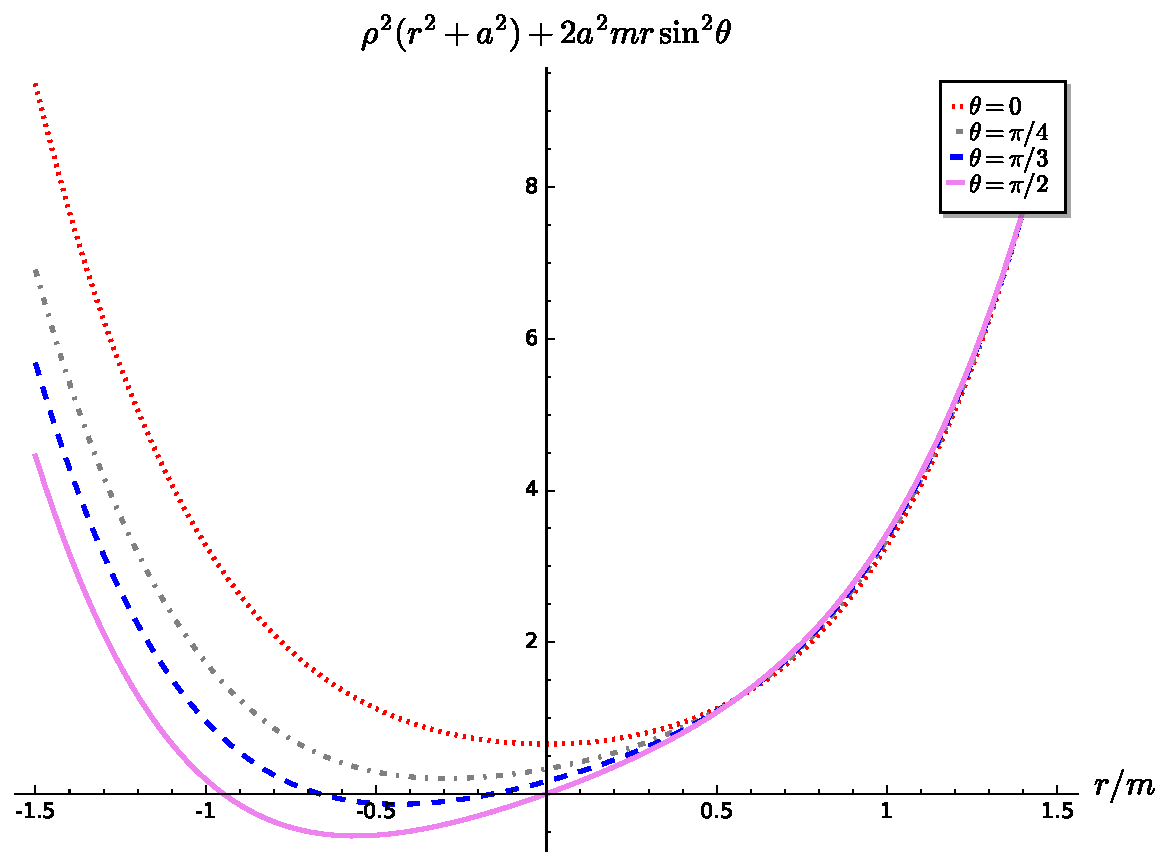
\includegraphics[width=0.7\textwidth]{ker_sign_gpp.pdf}}
\caption[]{\label{f:ker:sign_gpp} \footnotesize
Graph of the function giving the sign of $g_{\ph\ph}$ for $a=0.9m$
and various values of $\theta$.}
\end{figure}

\subsection{Carter time machine}

Let us now focus on the second Killing vector, $\w{\eta}$.
From (\ref{e:ker:metric_BL}) and (\ref{e:ker:def_rho2}), we have
\[
    \w{\eta}\cdot\w{\eta} = g_{\ph\ph} = \left( r^2 + a^2 + \frac{2 a^2 m r \sin^2\th}{r^2 + a^2\cos^2\th} \right) \sin^2\th .
\]
Hence
\[
    \w{\eta}\ \mbox{spacelike} \iff
        (r^2 + a^2)(r^2 + a^2\cos^2\th) + 2 a^2 m r \sin^2\th > 0 .
\]
For $\theta\rightarrow 0$ or $\theta\rightarrow\pi$, the left-hand side of the above equality
is always positive, but for $\theta=\pi/2$ and $r$ negative with $|r|$
small enough so that $2 a^2 m |r| > r^2(r^2 + a^2)$, it is negative. This feature
is apparent on Fig.~\ref{f:ker:sign_gpp}: for $\theta$ close to $\pi/2$,
there is a region $\mathscr{T}$ defined by $r_{\mathscr{T}}(\theta) < r < 0$ for some
negative function $r_{\mathscr{T}}(\theta)$, such that $g_{\ph\ph}<0$.
Since $\mathscr{T}$ corresponds to negative values of $r$, we have
$\mathscr{T}\subset \M_{\rm III}$.
Hence we conclude:
\begin{itemize}
\item $\w{\eta}$ is spacelike in all $\M_{\rm I}$ and $\M_{\rm II}$, as well
as outside the region $\mathscr{T}$ in $\M_{\rm III}$;
\item $\w{\eta}$ is timelike in the subset $\mathscr{T}$ of $\M_{\rm III}$;
\item $\w{\eta}$ is null at the boundary of $\mathscr{T}$.
\end{itemize}
The region $\mathscr{T}$ is called
\defin{Carter time machine}\index{Carter!time machine}\index{time!machine (Carter)}.
This name stems from the fact that thanks to $\mathscr{T}$, there is
a future-directed timelike curve connecting any two points of $\M_{\rm III}$
(see e.g. Proposition~2.4.7 of O'Neill's textbook \cite{ONeil95} for a
demonstration, or Carter's original article \cite{Carte68}).

\subsection{Singularities}

The components $g_{\alpha\beta}$ of the Kerr metric as given by  (\ref{e:ker:metric_BL})
are diverging at various locations:
\begin{itemize}
\item when $\rho^2\rightarrow 0$, which, given (\ref{e:ker:def_rho2})
and assuming $a\not=0$, is equivalent to approaching
the cylinder $\ring$ defined by (\ref{e:ker:def_ring});
\item when $\Delta\rightarrow 0$, which, given (\ref{e:ker:def_Delta}), is equivalent to either $r\rightarrow r_-$
or $r\rightarrow r_+$; the first case corresponds to the boundary (within $\R^2\times\SS^2$)
between $\M_{\rm II}$ and $\M_{\rm III}$ and the second case to the boundary
between $\M_{\rm I}$ and $\M_{\rm II}$.
\end{itemize}
The divergence when $\rho^2\rightarrow 0$ corresponds to a
\emph{curvature singularity}\index{curvature!singularity}\index{singularity!curvature --}.
Indeed the Kretschmann scalar of Kerr metric is (cf. Sec.~\ref{s:sam:Kerr_solution})
\be
    K := R_{\mu\nu\rho\sigma} R^{\mu\nu\rho\sigma}
     = 48 \frac{m^2}{\rho^{12}} \left( r^6 - 15 r^4 a^2\cos^2\th + 15 r^2 a^4 \cos^4\th - a^6\cos^6\th \right) .
\ee
The value for $\theta=\pi/2$ is thus $K = 48 m^2 / r^6$, which clearly diverges
for $r\rightarrow 0$ (i.e. $\rho^2\rightarrow 0$).
Hence $\ring$ is called the
\defin{ring singularity}\index{ring!singularity}\index{singularity!ring --}
of Kerr spacetime, the word \emph{ring} reflecting the fact that $t=\mathrm{const}$
sections of $\ring$ are $\SS^1$ circles [cf. Eq.~(\ref{e:ker:ring_R_S1})].

On the contrary, we shall see in the next section that the divergence
of the metric components when $\Delta\rightarrow 0$ corresponds to
a mere
\emph{coordinate singularity}\index{coordinate!singularity}\index{singularity!coordinate --},
i.e. to a pathology of Boyer-Lindquist coordinates, which can be cured by switching to
other coordinates.

\section{Kerr coordinates and extension of the spacetime manifold}

\subsection{Kerr coordinates}

The \defin{Kerr coordinates}\index{Kerr!coordinates} are coordinates
$\hat{x}^\alpha = (v,r,\th,\tph)$ defined on $\R^2\times\SS^2$ and related to the Boyer-Lindquist coordinates
$x^\alpha = (t,r,\th,\ph)$ introduced in Sec.~\ref{s:ker:expr_BL} by
\begin{subequations}
\label{e:ker:Kerr_coord}
\begin{align}
& \encadre{\D v = \D t + \frac{r^2+a^2}{\Delta} \, \D r} \label{e:ker:Kerr_coord_v}\\
& \encadre{\D \tph = \D \ph + \frac{a}{\Delta}\, \D r} . \label{e:ker:Kerr_coord_tph}
\end{align}
\end{subequations}
If $a=0$, we note that Kerr coordinates are nothing but the ingoing Eddington-Finkelstein
coordinates on Schwarzschild spacetime (cf. Sec.~??).

The components $\hat{g}_{\alpha\beta}$
of the metric tensor $\w{g}$ with respect to the Kerr coordinates
are computed from those with respect to the Boyer-Lindquist ones, as given
by Eq.~(\ref{e:ker:metric_BL}). One gets (cf. Appendix~\ref{s:sam} or
Eq.~(5.31) of Ref.~\cite{HawkiE73}, or Lemma~2.5.2 of \cite{ONeil95}):
\be \label{e:ker:metric_Kerr_coord}
    \begin{array}{ll}
    \hat{g}_{\mu\nu}\,  \D \hat{x}^\mu \D \hat{x}^\nu  = &
    \displaystyle - \left( 1 - \frac{2m r}{\rho^2} \right) \, \D v^2
    + 2 \D v\, \D r
    - \frac{4 a m  r \sin^2\th}{\rho^2} \,  \D v\, \D\tph \\[2ex]
    & - 2 a \sin^2\th \, \D r\, \D \tph  \displaystyle + \rho^2 \D \th^2
    + \left( r^2 + a^2 + \frac{2 a^2 m r \sin^2\th}{\rho^2} \right)
    \sin^2\th \, \D \tph^2 .
    \end{array}
\ee
We note that these metric components do not have any divergence when
$\Delta\rightarrow 0$, contrary to the Boyer-Lindquist ones. Hence, we may extend
the Kerr metric to the points of $\R^2\times\SS^2$ where $\Delta=0$, i.e.
to the hypersurfaces (cf. Fig.~\ref{f:ker:spher_view})
\be
    \Hor := \left\{ p \in \R^2\times\SS^2,\quad r(p) = r_+ \right\}
\ee
and
\be
    \Hor_{\rm in} := \left\{ p \in \R^2\times\SS^2,\quad r(p) = r_- \right\} .
\ee
The hypersurface $\Hor$ is actually the interface between the regions $\M_{\rm I}$
and $\M_{\rm II}$ and $\Hor_{\rm in}$ is the interface between $\M_{\rm II}$
and $\M_{\rm III}$ [cf. Eq.~(\ref{e:ker:M_I_III_r})].
We thus consider
\be
    \M := \M_{\rm BL} \cup \Hor \cup \Hor_{\rm in} = \R^2\times\SS^2 \setminus \ring
\ee
as the spacetime manifold. In order for $\w{g}$ defined by (\ref{e:ker:metric_Kerr_coord})
to be a well defined metric on $\M$, it does not suffices that the components
$\hat{g}_{\alpha\beta}$ do not diverge at $\Hor$ and $\Hor_{\rm in}$: one shall
check that $\w{g}$ is a non-degenerate bilinear form there as well.
This is easily proven by considering the determinant of the metric components,
which turns out to have a simple form (cf. Sec.~\ref{s:sam:Kerr_Kerr_coord}):
\be
    \det (\hat{g}_{\alpha\beta}) = -\rho^4 \sin^2\th .
\ee
Except at $\th=0$ and $\th=\pi$ (the usual singularity of spherical coordinates),
we have $\det (\hat{g}_{\alpha\beta}) \not= 0$ everywhere on $\M$, since
$\rho$ vanishes only on $\ring$, which is excluded from $\M$.
Hence we conclude that $\w{g}$ is not degenerate on $\M$ and thus
$(\M,\w{g})$ is a well behaved spacetime --- our \defin{Kerr spacetime}\index{Kerr!spacetime}
from now. We note that, contrary to $\M_{\rm BL}$, $\M$ is a connected manifold.

We deduce from (\ref{e:ker:Kerr_coord}) that the Kerr coordinate frame
is related to the Boyer-Lindquist coordinate frame by
\begin{subequations}
\label{e:ker:frame_Kerr_BL}
\begin{align}
    & \wpar_v = \wpar_t \\
    & \wpar_{\hat{r}} = \wpar_r - \frac{a^2+r^2}{\Delta} \wpar_t
                        - \frac{a}{\Delta} \wpar_\ph \\
    & \wpar_\th = \wpar_\th \\
    & \wpar_{\tph} = \wpar_\ph .
\end{align}
\end{subequations}
Note that we are using the notation $\wpar_{\hat{r}}$ for the $\partial/\partial r$
vector of the Kerr coordinates $\hat{x}^\alpha = (v,r,\th,\tph)$, to distinguish
it from the $\partial/\partial r$ vector of the Boyer-Lindquist coordinates.
We read on (\ref{e:ker:metric_Kerr_coord}) that $\hat{g}_{rr} = 0$, which
implies that $\wpar_{\hat{r}}$ is a null vector. Moreover, asymptotically,
\[
    \wpar_{\hat{r}} \sim \wpar_r - \wpar_t \quad\mbox{when}\
            r \rightarrow +\infty .
\]
This shows that $\wpar_{\hat{r}}$ is past-directed. Hence the field lines
of $-\wpar_{\hat{r}}$ are future-directed null curves,
which may be qualified of \emph{ingoing} since, by definition, $-\wpar_{\hat{r}}$ points towards
decreasing values of $r$. Note that, by the very definition of $\wpar_{\hat{r}}$,
the values of the coordinates $(v,\th,\tph)$ are fixed along each of these
null curves. We shall therefore denote them by $\Li^{\rm in}_{(v,\th,\tph)}$.
We shall see below that $\Li^{\rm in}_{(v,\th,\tph)}$ is actually a null geodesic.


\begin{hist}
Kerr coordinates are actually those in which R.P.~Kerr originally presented his
solution \cite{Kerr63}. Actually, he used $-\tph$ instead of $\tph$; hence
the correspondance between our notations and those of Kerr's article \cite{Kerr63}
is $v\leftrightarrow u$ and $\tph\leftrightarrow -\phi$.
\end{hist}

\subsection{3+1 Kerr coordinates}

As in Sec.~??, we shall move from the null coordinate $v$ to a (asymptotically)
timelike one by setting
\be \label{e:ker:def_t_tilde}
    \encadre{\ti = v - r} \iff \encadre{v = \ti + r}
\ee
so that $v$ appears as the advanced time $\ti+v$ (compare Eq.~(??)). We thus consider
the coordinates
\be
    (\tilde{x}^\alpha) = (\ti, r, \th,\tph) ,
\ee
which we call the
\defin{3+1 Kerr coordinates}\index{3+1!Kerr coordinates}\index{Kerr!coordinates!3+1 --}.
In it worth to relate them to the Boyer-Lindquist coordinates
$(t,r,\th,\ph)$. This is easily done
by combining (\ref{e:ker:Kerr_coord}) with $\D\ti = \D v - \D r$:
\begin{subequations}
\label{e:ker:Kerr_3p1_BL}
\begin{align}
& \encadre{\D \ti = \D t + \frac{2m r}{\Delta} \, \D r} \\
& \encadre{\D \tph = \D \ph + \frac{a}{\Delta}\, \D r} .
\end{align}
\end{subequations}


\begin{hist}
In the historical article \cite{Kerr63}, R.P.~Kerr introduced $\ti$ by exactly
the same transformation as (\ref{e:ker:def_t_tilde}) ($\ti$ is denoted $t$
in \cite{Kerr63}), but along with Cartesian-type coordinates $(x,y,z)$
deduced from $(r,\th,\tph)$ by spheroidal transformations, to form the 3+1
coordinate system $(\ti,x,y,z)$, which is today known as
\defin{Kerr-Schild coordinates}\index{Kerr-Schild coordinates} (despite
they have been introduced first in Kerr's article \cite{Kerr63} (1963) and not
in the article by Kerr and Schild \cite{KerrS65} (1965)). Accordingly,
our ``3+1 Kerr coordinates'' are a mix of the original Kerr coordinates
$(v,r,\th,\tph)$ (cf. the previous historical note)
and the Kerr-Schild coordinates $(\ti,x,y,z)$.
\end{hist}

Since the transform (\ref{e:ker:def_t_tilde}) leads to $\D v = \D\ti + \D r$,
the metric components $\tilde{g}_{\alpha\beta}$ with respect to the
3+1 coordinates $(\ti,r,\th,\tph)$ are easily deduced from
(\ref{e:ker:metric_Kerr_coord}):
\be \label{e:ker:metric_Kerr_3p1}
    \encadre{
    \begin{array}{ll}
    \tilde{g}_{\mu\nu}\,  \D \tilde{x}^\mu \D \tilde{x}^\nu  = &
    \displaystyle - \left( 1 - \frac{2m r}{\rho^2} \right)  \D \ti^2
    + \frac{4m r}{\rho^2} \D\ti\, \D r
    - \frac{4 a m  r \sin^2\th}{\rho^2} \,  \D \ti\, \D\tph \\[2ex]
    &\displaystyle  + \left( 1 + \frac{2m r}{\rho^2} \right) \D r^2
     - 2 a \left( 1 + \frac{2m r}{\rho^2} \right) \sin^2\th \, \D r\, \D \tph \\[2ex]
    & \displaystyle + \rho^2 \D \th^2
    + \left( r^2 + a^2 + \frac{2 a^2 m r \sin^2\th}{\rho^2} \right)
    \sin^2\th \, \D \tph^2 .
    \end{array}
    }
\ee
As a check, we notice the agreement with Eq.~(D.4) of Ref.~\cite{GourgJ06}.

Since we kept $r$, $\th$ and $\tph$ and simply changed
$v$ to $\ti$ via (\ref{e:ker:def_t_tilde}) when moving from the Kerr
coordinates to the 3+1 Kerr coordinates, we easily get the relation
between the two coordinate frames:
\begin{subequations}
\label{e:ker:frame_Kerr3p1_Kerr}
\begin{align}
    & \wpar_\ti = \wpar_v \\
    & \wpar_{\tilde r} = \wpar_v + \wpar_{\hat{r}} \\
    & \wpar_\th = \wpar_\th \\
    & \wpar_\tph = \wpar_\ph .
\end{align}
\end{subequations}
Note that we have denoted by $\wpar_{\tilde r}$ the second vector of the
coordinate frame associated to the 3+1 Kerr coordinates
$(\tilde{x}^\alpha) = (\ti, r, \th,\tph)$, in order to distinguish it from
the coordinate vector $\wpar_{\hat r}$ of the Kerr coordinates
$(\hat{x}^\alpha) = (v, r, \th,\tph)$, as well as from the coordinate vector
$\wpar_r$ of the Boyer-Lindquist coordinates
$(x^\alpha) = (t,r,\th,\ph)$.

By combining (\ref{e:ker:frame_Kerr_BL}) and (\ref{e:ker:frame_Kerr3p1_Kerr}),
we get the relation between the 3+1 Kerr coordinate frame and the
Boyer-Lindquist coordinate frame:
\begin{subequations}
\label{e:ker:frame_Kerr3p1_BL}
\begin{align}
    & \wpar_\ti = \wpar_t \label{e:ker:frame_Kerr3p1_BL_t} \\
    & \wpar_{\tilde r} = \wpar_r - \frac{2mr}{\Delta} \wpar_t
                        - \frac{a}{\Delta} \wpar_\ph \\
    & \wpar_\th = \wpar_\th \\
    & \wpar_{\tph} = \wpar_\ph . \label{e:ker:frame_Kerr3p1_BL_ph}
\end{align}
\end{subequations}
We notice on (\ref{e:ker:frame_Kerr3p1_BL_t}) and (\ref{e:ker:frame_Kerr3p1_BL_ph})
that the coordinate frame vectors $\wpar_\ti$ and $\wpar_\tph$
coincide with the Killing vectors $\w{\xi}$ and $\w{\eta}$:
\be \label{e:ker:Killing_vec_3p1}
    \encadre{\wpar_\ti = \w{\xi}} \quad \mbox{and} \quad
    \encadre{\wpar_\tph = \w{\eta}} .
\ee
That $\wpar_\ti$ and $\wpar_\tph$ are Killing vectors is not surprising since
the metric components (\ref{e:ker:metric_Kerr_3p1}) do not depend on $\ti$
nor on $\tph$.

The determinant of the metric components (\ref{e:ker:metric_Kerr_3p1}) has
a very simple form (cf. Sec.~\ref{s:sam:Kerr_Kerr_coord} for the computation):
\be \label{e:ker:det_g_3p1}
    \det\left( \tilde{g}_{\mu\nu} \right) = - \rho^4\sin^2\th .
\ee
The inverse metric takes also a rather simple form in terms of the 3+1
Kerr coordinates (cf. Sec.~\ref{s:sam:Kerr_Kerr_coord} for the computation):
\be \label{e:ker:inv_met_3p1}
    \tilde{g}^{\alpha\beta} = \left(
    \begin{array}{cccc}
    - \left( 1 + \frac{2m r}{\rho^2} \right) & \frac{2m r}{\rho^2} & 0 & 0 \\[1ex]
    \frac{2m r}{\rho^2} & \frac{\Delta}{\rho^2} & 0 & \frac{a}{\rho^2} \\[1ex]
    0 & 0 &\frac{1}{\rho^2} & 0 \\[1ex]
    0 & \frac{a}{\rho^2} & 0 & \frac{1}{\rho^2\sin^2\th}
    \end{array}
    \right) .
\ee

Comparing (\ref{e:ker:frame_Kerr3p1_BL}) with (\ref{e:ker:metric_BL}), we
note that the metric components in 3+1 Kerr coordinates are slightly more
complicated than those in Boyer-Lindquist coordinates, for they contain
extra non-diagonal terms: ${\tilde g}_{\ti r}$ and ${\tilde g}_{r \tph}$. However
the determinant (\ref{e:ker:det_g_3p1})
and the inverse metric (\ref{e:ker:inv_met_3p1}) are pretty simple. Morever
the 3+1 Kerr coordinates are as well adapted to the spacetime symmetries
as the Boyer-Lindquist ones, as (\ref{e:ker:Killing_vec_3p1}) shows, and
they have the great advantage to be regular on the boundary hypersurfaces
$\Hor$ and $\Hor_{\rm in}$, contrary to the Boyer-Lindquist ones.
The last feature is all the more important since
$\Hor$ is the future event horizon of Kerr spacetime,
as we are going to see.
Therefore, we shall continue our study of Kerr spacetime, and especially the
black hole aspect, by means of the 3+1 Kerr coordinates.

%%%%%%%%%%%%%%%%%%%%%%%%%%%%%%%%%%%%%%%%%%%%%%%%%%%%%%%%%%%%%%%%%%%%%%%%%%%%%%%

\section{Event horizon}

\subsection{Killing horizons} \label{s:ker:Killing_hor}

Let us consider the hypersurfaces of $\M$ defined by a fixed value of
the coordinate $r$. $\Hor$ and $\Hor_{\rm in}$ are two particular cases,
corresponding to $r=r_+$ and $r=r_-$ respectively.
The normal 1-form to these hypersurfaces is $\dd r$; the corresponding
gradient vector field is $\vw{\nabla} r$, the components of which are
$\nabla^\alpha r = g^{\alpha\mu} \partial_\mu r = g^{\alpha r}$.
According to (\ref{e:ker:inv_met_3p1}), we have
\be \label{e:ker:nab_r_comp}
    \nabla^\alpha r = \left( \frac{2m r}{\rho^2}, \frac{\Delta}{\rho^2}, 0, \frac{a}{\rho^2}
            \right) .
\ee
It is then quite natural to consider the vector field
\be
    \w{n} := \rho^2 \vw{\nabla} r
\ee
for the normal to the hypersurfaces $r=\mathrm{const}$. According to (\ref{e:ker:nab_r_comp}),
it has indeed simple components on the 3+1 Kerr frame:
\be \label{e:ker:normal_r}
    \w{n} = 2 m r \, \wpar_\ti + \Delta \, \wpar_{\tilde r} + a \, \wpar_\tph .
\ee
The scalar square of $\w{n}$ is
\[
    \w{n}\cdot\w{n} = \w{g}(\w{n},\w{n}) = n_\mu n^\mu = \rho^2 (\nabla_\mu r) n^\mu
    = \rho^2 n^r .
\]
Hence, in view of (\ref{e:ker:normal_r}),
\be
    \w{n}\cdot\w{n} = \rho^2 \Delta .
\ee
Since $\rho^2>0$ everywhere on $\M$ and $\Delta = (r-r_+)(r-r_-)$ [cf. Eq.~(\ref{e:ker:def_Delta})], we conclude that
\begin{itemize}
\item the hypersurfaces $r=\mathrm{const}$ are timelike in regions $\M_{\rm I}$ and $\M_{\rm III}$;
\item the hypersurfaces $r=\mathrm{const}$ are spacelike in region $\M_{\rm II}$;
\item $\Hor$ (where $r=r_+$) and $\Hor_{\rm in}$ (where $r=r_-$) are null hypersurfaces.
\end{itemize}

On $\Hor$ and $\Hor_{\rm in}$, $\Delta=0$, so that (\ref{e:ker:nab_r_comp})
reduces to
\be \label{e:ker:normal_r_Killing}
    \w{n} = 2 m r_{\pm} \, \wpar_\ti + a \, \wpar_\tph = 2 m r_{\pm} \, \w{\xi}
        + a \, \w{\eta} ,
\ee
where we have used (\ref{e:ker:Killing_vec_3p1}) and $r_{\pm}$ stands for
$r_+$ on $\Hor$ and $r_-$ on $\Hor_{\rm in}$.
On $\Hor$, we may rewrite this expression as
\be \label{e:ker:n_rp_chi}
    \w{n} = 2 m r_+ \, \w{\chi} ,
\ee
with
\be \label{e:ker:def_chi}
    \encadre{\w{\chi} := \w{\xi} + \Omega_H \, \w{\eta} }
\ee
and
\be \label{e:ker:def_OmegaH}
    \encadre{\Omega_H := \frac{a}{2 m r_+} = \frac{a}{r_+^2 + a^2}
        = \frac{a}{2m\left( m + \sqrt{m^2-a^2} \right)} }.
\ee
$\Omega_H$ being a constant, the vector field $\w{\chi}$ defined by
(\ref{e:ker:def_chi}) is a Killing vector field. Moreover, (\ref{e:ker:n_rp_chi})
shows that this Killing vector is normal to the null hypersurface $\Hor$.
We conclude that $\Hor$ is a
Killing horizon\index{Killing!horizon}\index{horizon!Killing --} (cf. Sec.~\ref{s:def:def_Killing_hor}).

Similarly, on $\Hor_{\rm in}$, we may rewrite (\ref{e:ker:normal_r_Killing})
as $\w{n} = 2 m r_- \, \w{\chi}_{\rm in}$, with
\be
    \w{\chi}_{\rm in} := \w{\xi} + \Omega_{\rm in} \, \w{\eta}
\ee
and
\be
    \Omega_{\rm in} := \frac{a}{2 m r_-} = \frac{a}{r_-^2 + a^2}
        = \frac{a}{2m\left( m - \sqrt{m^2-a^2} \right)} ,
\ee
thereby arriving at the same conclusion: $\Hor_{\rm in}$ is a Killing horizon.

\subsection{Event horizon}

As a null hypersurface, $\Hor$ is a one-way membrane (cf. Sec.~\ref{s:def:hor_as_null}),
therefore any (massive or null) particle that crossed it from $\M_{\rm I}$ to
$\M_{\rm II}$ can never be back in $\M_{\rm I}$.
Thus $\M_{\rm II}$ and $\M_{\rm III}$ are in the black hole region with respect to
$\scri^+$ corresponding to $r\rightarrow +\infty$.

Let us show that $\Hor$ is exactly the boundary of the black hole region, i.e.
that any point in $\M_{\rm I}$ can emit a signal reaching $\scri^+$.
To this aim, let us consider the vector field $\wl$ defined on $\M$ by
\be \label{e:ker:def_ell_outgoing}
    \wl = \left( \frac{1}{2} + \frac{m r}{r^2 + a^2} \right) \wpar_\ti
        + \left( \frac{1}{2} - \frac{m r}{r^2 + a^2} \right) \wpar_{\tilde r}
        + \frac{a}{r^2+a^2} \, \wpar_\tph .
\ee
$\wl$ is a null vector everywhere, as it can easily be checked
via (\ref{e:ker:metric_Kerr_3p1}):
\be
    \w{g}(\wl,\wl) = 0 .
\ee
The field lines of $\wl$ are thus null curves\footnote{They are actually
null geodesics, as we shall see in Sec.~\ref{s:ker:surf_grav}.}. They obey
\[
   \frac{\D r}{\D\lambda} = \el^r = \frac{1}{2} - \frac{m r}{r^2 + a^2} ,
\]
where $\lambda$ is the parameter associated with $\wl$.
Let $p$ be a point in $\M_{\rm I}$, of 3+1 Kerr coordinates $(\ti_0,r_0,\th_0,\tph_0)$.
The null curve $\Li$ of tangent vector $\wl$ that departs from $p$ obeys
\[
    \left. \frac{\D r}{\D\lambda} \right| _{p} = \frac{1}{2} - \frac{m r_0}{r_0^2 + a^2} > 0 ,
\]
where the inequality follows from the fact that $r_0 > r_+$ wherever $p$ lies in
$\M_{\rm I}$.
Hence, initially $r$ is increasing along $\Li$ and we get, since $-mr/(r^2+a^2)$ is an
increasing function of $r$,
\[
    \frac{\D r}{\D\lambda} > \frac{1}{2} - \frac{m r_0}{r_0^2 + a^2} =: \alpha .
\]
Since $\alpha$ is a constant, we deduce that
\[
    r > r_0 + \alpha(\lambda - \lambda_0) ,
\]
where $\lambda_0$ is the value of $\Li$'s parameter at $p$. When $\lambda\rightarrow +\infty$,
we get $r\rightarrow +\infty$, which proves that the null curve $\Li$
reaches $\scri^+$. Hence we conclude:
\begin{quote}
$\mathscr{B} = \M \setminus \M_{\rm I}$ is the black hole region, the event
horizon of which is $\Hor$.
\end{quote}
Incidentally, this illustrates Hawking's strong rigidity theorem discussed
in Sec.~\ref{s:glo:strong_rigidity}: the event horizon of Kerr spacetime
is indeed a Killing horizon, as we have shown in Sec.~\ref{s:ker:Killing_hor}.

According to the discussion in Sec.~\ref{s:glo:strong_rigidity}, we may then
call the quantity $\Omega_H$ introduced in
Eqs.~(\ref{e:ker:def_chi})-(\ref{e:ker:def_OmegaH}) the
\defin{black hole rotation velocity}\index{black hole!rotation velocity}\index{rotation!velocity}.


\subsection{Surface gravity} \label{s:ker:surf_grav}

By construction, the null vector field $\wl$ defined by Eq.~(\ref{e:ker:def_ell_outgoing}) coincides with the Killing vector $\w{\chi}$ on $\Hor$,
since $m r/(r^2 + a^2) \equalH 1/2$ and $a/(r^2+a^2) \equalH \Omega_H$:
\be
    \wl \equalH \w{\chi} .
\ee
Moreover, $\wl$ is a pregeodesic vector (cf. Sec.~\ref{s:def:geod_gener}) everywhere.
An explicit computation (cf. Sec.~\ref{s:sam:Kerr_Kerr_coord}) reveals that
\be \label{e:ker:pregeod_ell}
    \wnab_{\wl}\, \wl = \bar{\kappa} \, \wl ,
\ee
with
\be
    \bar{\kappa} := \frac{m(r^2-a^2)}{(r^2+a^2)^2} .
\ee
As we have seen in Sec.~\ref{s:def:geod_gener}, Eq.~(\ref{e:ker:pregeod_ell})
 implies that the field
lines of $\wl$ are null geodesics. Actually they constitute a privileged
family of null geodesics in Kerr spacetime, called the
\defin{outgoing principal null geodesics}\index{principal!null geodesic}.

Since $\wl$ coincides with $\w{\chi}$ on $\Hor$, we have
\be \label{e:ker:pregeod_chi}
    \encadre{ \wnab_{\w{\chi}}\, \w{\chi} \equalH \kappa \, \w{\chi} },
\ee
with
\[
    \kappa = \left. \bar{\kappa} \right| _{r=r_+} = \frac{m(r_+^2-a^2)}{(r_+^2+a^2)^2} .
\]
$r_+$ being a zero of $\Delta$, we have $r_+^2 + a^2 = 2 m r_+$, so that we may
rewrite the above expression in terms of $r_+$ and $a$ only:
\be
    \kappa = \frac{r_+^2 - a^2}{2r_+(r_+^2+a^2)} .
\ee
Substituting (\ref{e:ker:def_r_pm}) for $r_+$, we get an expression in terms
of the two basic Kerr parameters:
\be
    \encadre{ \kappa = \frac{\sqrt{m^2 - a^2}}{2m(m + \sqrt{m^2-a^2})} } .
\ee
From Eq.~(\ref{e:ker:pregeod_chi}), $\kappa$ is the non-affinity coefficient
of the null normal $\chi$ of the null hypersurface $\Hor$. In the present
context, where $\Hor$ is an event horizon, $\kappa$ is called
the \defin{black hole surface gravity}\index{surface!gravity}\index{gravity!surface --}.

%%%%%%%%%%%%%%%%%%%%%%%%%%%%%%%%%%%%%%%%%%%%%%%%%%%%%%%%%%%%%%%%%%%%%%%%%%%%%%%

\section{Global quantities}

\subsection{Mass}

\subsection{Angular momentum}

\subsection{Black hole area}

%%%%%%%%%%%%%%%%%%%%%%%%%%%%%%%%%%%%%%%%%%%%%%%%%%%%%%%%%%%%%%%%%%%%%%%%%%%%%%%

\section{Maximal extension}

\subsection{Cauchy horizon}
